\chapter{Dobór parametrów regulacji}

W celu dobrania parametrów regulacji algorytmu DMC wykonano serię symulacji, w których przebieg wartości zadanej $Y^{zad}(k)$ miał postać skoku z wartości \num{0} do wartości \num{1} w chwili odpowiadającej 21 próbce w zakresie 400 próbek procesu. Sygnał zakłocenia $Z(k)$ miał wartość \num{0} dla każdej chwili $k$.

Za wartości początkowe parametrów regulatora przyjęto $D=N=201$ , $N_u = 200$ , $\lambda =$ \num{1.0}. Dla kolejnych symulacji modyfikowano wartość parametru $N_u$ obserwując zmianę wskaźnika jakości $e$ oraz przebieg sygnału. Wykonano sześć symulacji dla parametru $N_u$ = 2, 3, 4, 5, 6, 200. Wyniki przebiegów zestawiono ze sobą (Rys. \ref{Nu}), wartość wskaźnika jakości $e$ zebrano w tabeli (Tab. \ref{eNu}).

\begin{table}
	[b] \caption{Wartość wskaźnika $e$ jakości dla różnych wartości parametru $N_u$}
	\label{eNu}
	\centering
	\sisetup{table-format = 2.4}
	\begin{small}
		\begin{tabular}{|c|c|}
			\hline 
			Horyzont sterowania $N_u$ & Błąd średniokwadratowy $e$ \\ 
			\hline 
			200 & \num{6.0032} \\ 
			\hline 
			2 & \num{6.6227} \\ 
			\hline 
			3 & \num{5.6199} \\ 
			\hline 
			4 & \num{5.4694} \\ 
			\hline 
			5 & \num{5.5429} \\ 
			\hline 
			6 & \num{5.6802} \\ 
			\hline 
		\end{tabular}
	\end{small}
\end{table}

Wyraźnie widać, że najlepszy rezultat pod kątem minimalizacji wskaźnika jakości daje $N_u$~=~4. Przebieg procesu dla tej wartości mimo iż nie jest całkowicie gładki, nie wpada w oscylacje i może być uznany za zadawalający.

\begin{figure}
	
	\centering
	\caption{ Przebieg symulacji algorytmu DMC dla różnych wartości  parametru $N_u$ }
	% This file was created by matlab2tikz.
%
%The latest updates can be retrieved from
%  http://www.mathworks.com/matlabcentral/fileexchange/22022-matlab2tikz-matlab2tikz
%where you can also make suggestions and rate matlab2tikz.
%
\definecolor{mycolor1}{rgb}{0.00000,0.44700,0.74100}%
\definecolor{mycolor2}{rgb}{0.85000,0.32500,0.09800}%
\definecolor{mycolor3}{rgb}{0.92900,0.69400,0.12500}%
\definecolor{mycolor4}{rgb}{0.49400,0.18400,0.55600}%
\definecolor{mycolor5}{rgb}{0.46600,0.67400,0.18800}%
\definecolor{mycolor6}{rgb}{0.30100,0.74500,0.93300}%
%
\begin{tikzpicture}

\begin{axis}[%
width=4.521in,
height=3.566in,
at={(0.758in,0.481in)},
scale only axis,
xmin=0,
xmax=100,
xlabel style={font=\color{white!15!black}},
xlabel={k},
ymin=0,
ymax=1,
ylabel style={font=\color{white!15!black}},
ylabel={U},
axis background/.style={fill=white},
axis x line*=bottom,
axis y line*=left,
legend style={legend cell align=left, align=left, draw=white!15!black}
]
\addplot[const plot, color=mycolor1] table[row sep=crcr] {%
1	0\\
2	0\\
3	0\\
4	0\\
5	0\\
6	0\\
7	0\\
8	0\\
9	0\\
10	0\\
11	0\\
12	0\\
13	0\\
14	0\\
15	0\\
16	0\\
17	0\\
18	0\\
19	0\\
20	0\\
21	0\\
22	0\\
23	0\\
24	0\\
25	0.102102811945484\\
26	0.238305675353849\\
27	0.375472450520407\\
28	0.499054751339927\\
29	0.593670308725784\\
30	0.662512012651148\\
31	0.712987003403397\\
32	0.751686039564194\\
33	0.784256104523638\\
34	0.813459492112764\\
35	0.840088231310461\\
36	0.864077651456633\\
37	0.885092459326203\\
38	0.903008117709287\\
39	0.918005880429657\\
40	0.930469315575202\\
41	0.940858685078025\\
42	0.9495991837599\\
43	0.957026079744358\\
44	0.963380538095846\\
45	0.968830233661045\\
46	0.97349725430174\\
47	0.977480524618346\\
48	0.980868375831457\\
49	0.983743004195152\\
50	0.986180192607552\\
51	0.988247554504469\\
52	0.990003318757648\\
53	0.991496302759692\\
54	0.992766890040793\\
55	0.993848497004692\\
56	0.994769047967241\\
57	0.995552181896836\\
58	0.996218116381772\\
59	0.996784223969602\\
60	0.997265423385424\\
61	0.997674477472602\\
62	0.998022255034574\\
63	0.998317979567336\\
64	0.998569465780087\\
65	0.998783336164801\\
66	0.998965210438728\\
67	0.999119865152967\\
68	0.999251365241129\\
69	0.999363171936887\\
70	0.999458232137156\\
71	0.999539053595614\\
72	0.999607769124262\\
73	0.999666191858872\\
74	0.999715862878937\\
75	0.999758092077849\\
76	0.999793993038679\\
77	0.999824512647112\\
78	0.999850456166138\\
79	0.999872508460428\\
80	0.999891251986395\\
81	0.999907182072131\\
82	0.999920719918547\\
83	0.999932223672269\\
84	0.999941997857136\\
85	0.999950301403507\\
86	0.999957354478802\\
87	0.99996334429461\\
88	0.999968430042068\\
89	0.999972747086215\\
90	0.999976410531266\\
91	0.999979518251923\\
92	0.999982153471266\\
93	0.999984386953288\\
94	0.999986278867691\\
95	0.999987880375818\\
96	0.999989234979293\\
97	0.999990379666783\\
98	0.999991345889058\\
99	0.999992160388047\\
100	0.999992845901784\\
};
\addlegendentry{$\text{N}_{\text{u}}\text{=2}$}

\addplot[const plot, color=mycolor2] table[row sep=crcr] {%
1	0\\
2	0\\
3	0\\
4	0\\
5	0\\
6	0\\
7	0\\
8	0\\
9	0\\
10	0\\
11	0\\
12	0\\
13	0\\
14	0\\
15	0\\
16	0\\
17	0\\
18	0\\
19	0\\
20	0\\
21	0\\
22	0\\
23	0\\
24	0\\
25	0.152830579839198\\
26	0.361723685979986\\
27	0.567813252929803\\
28	0.740934525440941\\
29	0.847095360437015\\
30	0.893658115143514\\
31	0.90255973864811\\
32	0.895570671873684\\
33	0.89163036498361\\
34	0.898990405246294\\
35	0.91685828271975\\
36	0.939887677878803\\
37	0.961615803129477\\
38	0.977621370527924\\
39	0.986602460199098\\
40	0.989773437013205\\
41	0.989641380644215\\
42	0.988689847199495\\
43	0.988533654813312\\
44	0.989704626042417\\
45	0.991892848316057\\
46	0.994401945347177\\
47	0.996573965969035\\
48	0.998037076898529\\
49	0.998753666950623\\
50	0.998924656597726\\
51	0.998838350857697\\
52	0.998740665168325\\
53	0.998766808279368\\
54	0.998937329483177\\
55	0.999196697549384\\
56	0.999464818354491\\
57	0.999678006297738\\
58	0.999808372281484\\
59	0.999862529279366\\
60	0.999867769339971\\
61	0.999855454910885\\
62	0.999848800913543\\
63	0.999857968169211\\
64	0.999881621834702\\
65	0.999912037309881\\
66	0.999940598025195\\
67	0.999961538784302\\
68	0.999973216807206\\
69	0.999977361349574\\
70	0.999977327623101\\
71	0.999976368399375\\
72	0.999976556980123\\
73	0.999978522354457\\
74	0.999981799158156\\
75	0.999985440953475\\
76	0.999988577040411\\
77	0.999990730653257\\
78	0.99999187053213\\
79	0.999992275801492\\
80	0.999992333120867\\
81	0.99999236613075\\
82	0.999992548519416\\
83	0.999992902381439\\
84	0.999993351510946\\
85	0.999993790164412\\
86	0.999994136571704\\
87	0.999994357305398\\
88	0.999994464385011\\
89	0.999994496292151\\
90	0.999994495860299\\
91	0.999994494377281\\
92	0.999994505516522\\
93	0.999994527765157\\
94	0.999994551375948\\
95	0.999994565659013\\
96	0.999994563834085\\
97	0.999994544575335\\
98	0.999994510910527\\
99	0.999994467862375\\
100	0.999994420170427\\
};
\addlegendentry{$\text{N}_{\text{u}}\text{=4}$}

\addplot[const plot, color=mycolor3] table[row sep=crcr] {%
1	0\\
2	0\\
3	0\\
4	0\\
5	0\\
6	0\\
7	0\\
8	0\\
9	0\\
10	0\\
11	0\\
12	0\\
13	0\\
14	0\\
15	0\\
16	0\\
17	0\\
18	0\\
19	0\\
20	0\\
21	0\\
22	0\\
23	0\\
24	0\\
25	0.133897173815572\\
26	0.321115206483482\\
27	0.511631264994931\\
28	0.678383595193014\\
29	0.792226395557322\\
30	0.855526173038144\\
31	0.883011155485141\\
32	0.890940478023966\\
33	0.894488786073082\\
34	0.902001327932616\\
35	0.915415800451548\\
36	0.932795450824833\\
37	0.950546348943912\\
38	0.965588569427341\\
39	0.976386281354062\\
40	0.982949900502618\\
41	0.986333207908015\\
42	0.987935247191869\\
43	0.988944640633582\\
44	0.990071774460171\\
45	0.99153767783847\\
46	0.993227134232591\\
47	0.99488961042946\\
48	0.996300170273974\\
49	0.997343166459794\\
50	0.998021635622631\\
51	0.99841949413223\\
52	0.998649038448985\\
53	0.998807997981494\\
54	0.998957372967232\\
55	0.999119622222437\\
56	0.999289890867172\\
57	0.999451394344361\\
58	0.999588170356415\\
59	0.999691997054804\\
60	0.999763533953464\\
61	0.999809679061184\\
62	0.999839618931836\\
63	0.999861493436462\\
64	0.99988060805865\\
65	0.99989921587894\\
66	0.999917339137214\\
67	0.999933951674584\\
68	0.999947987829233\\
69	0.999958913662965\\
70	0.999966849571879\\
71	0.999972389428293\\
72	0.999976305706428\\
73	0.99997929204983\\
74	0.999981820329698\\
75	0.999984118423404\\
76	0.999986230487926\\
77	0.999988108053999\\
78	0.999989689995482\\
79	0.999990949707531\\
80	0.999991907473925\\
81	0.999992618530584\\
82	0.999993151288431\\
83	0.999993567631283\\
84	0.99999391162188\\
85	0.999994207452691\\
86	0.999994463911343\\
87	0.999994681439297\\
88	0.999994858501267\\
89	0.999994995498664\\
90	0.999995095981206\\
91	0.999995165912693\\
92	0.999995212093284\\
93	0.999995240674294\\
94	0.999995256284039\\
95	0.999995261857448\\
96	0.999995258976811\\
97	0.999995248427253\\
98	0.999995230710908\\
99	0.999995206376599\\
100	0.999995176139262\\
};
\addlegendentry{$\text{N}_{\text{u}}\text{=6}$}

\addplot[const plot, color=mycolor4] table[row sep=crcr] {%
1	0\\
2	0\\
3	0\\
4	0\\
5	0\\
6	0\\
7	0\\
8	0\\
9	0\\
10	0\\
11	0\\
12	0\\
13	0\\
14	0\\
15	0\\
16	0\\
17	0\\
18	0\\
19	0\\
20	0\\
21	0\\
22	0\\
23	0\\
24	0\\
25	0.141216291560086\\
26	0.335135280647484\\
27	0.528772551560698\\
28	0.694909299141412\\
29	0.803486291289657\\
30	0.859671095829643\\
31	0.881007195275332\\
32	0.885287767972446\\
33	0.888321408492131\\
34	0.897687456964388\\
35	0.91391289454767\\
36	0.933786710700225\\
37	0.95290874574733\\
38	0.968050869605059\\
39	0.978039958830872\\
40	0.983453769232762\\
41	0.985857146511849\\
42	0.986936172692258\\
43	0.98791088660081\\
44	0.989341939727254\\
45	0.991232151434318\\
46	0.993279846019605\\
47	0.995135143667822\\
48	0.996565928939156\\
49	0.997512255909105\\
50	0.998054235735977\\
51	0.998339533297242\\
52	0.998513082951352\\
53	0.998673631227118\\
54	0.998862439205608\\
55	0.999075830409067\\
56	0.999287920337992\\
57	0.9994715843396\\
58	0.999611015116114\\
59	0.999704811710837\\
60	0.999762322963828\\
61	0.999797286027658\\
62	0.999822159811217\\
63	0.99984495373437\\
64	0.999868740941275\\
65	0.999893003389901\\
66	0.999915631236152\\
67	0.999934623984392\\
68	0.999949018778297\\
69	0.999959031244828\\
70	0.999965678938676\\
71	0.999970233934897\\
72	0.999973774022909\\
73	0.999976959255309\\
74	0.99998002908541\\
75	0.999982937534482\\
76	0.999985526359288\\
77	0.999987661487532\\
78	0.99998930013541\\
79	0.999990493294671\\
80	0.999991349257547\\
81	0.999991987443096\\
82	0.999992503551662\\
83	0.99999295460209\\
84	0.99999336181828\\
85	0.999993723664035\\
86	0.999994030660642\\
87	0.999994276223024\\
88	0.999994461398351\\
89	0.999994594367198\\
90	0.99999468707087\\
91	0.999994751400729\\
92	0.999994796563236\\
93	0.999994828163162\\
94	0.99999484870735\\
95	0.999994858831075\\
96	0.999994858557836\\
97	0.99999484815657\\
98	0.999994828470798\\
99	0.99999480082823\\
100	0.999994766743177\\
};
\addlegendentry{$\text{N}_{\text{u}}\text{=3}$}

\addplot[const plot, color=mycolor5] table[row sep=crcr] {%
1	0\\
2	0\\
3	0\\
4	0\\
5	0\\
6	0\\
7	0\\
8	0\\
9	0\\
10	0\\
11	0\\
12	0\\
13	0\\
14	0\\
15	0\\
16	0\\
17	0\\
18	0\\
19	0\\
20	0\\
21	0\\
22	0\\
23	0\\
24	0\\
25	0.146099355618009\\
26	0.347082950012633\\
27	0.547329610219117\\
28	0.717923304156553\\
29	0.826765425156101\\
30	0.879459696199112\\
31	0.895264391158991\\
32	0.893846050220434\\
33	0.892674163345827\\
34	0.900009712431596\\
35	0.916105901843892\\
36	0.936940628815679\\
37	0.957169804526246\\
38	0.972886078757048\\
39	0.982672955832442\\
40	0.987245424420625\\
41	0.988519363933043\\
42	0.988547344063404\\
43	0.988789314928265\\
44	0.989871172461661\\
45	0.991716656716522\\
46	0.993874301269228\\
47	0.995849442315995\\
48	0.997319055342042\\
49	0.998199499300323\\
50	0.99859910486088\\
51	0.998716863481079\\
52	0.998744919609282\\
53	0.998808791681461\\
54	0.998952843793722\\
55	0.999159368642301\\
56	0.999381864345807\\
57	0.999575341309258\\
58	0.99971403788827\\
59	0.99979506542223\\
60	0.999832104401258\\
61	0.999845264578098\\
62	0.999852265243106\\
63	0.999863649440795\\
64	0.999882256347604\\
65	0.999905553258005\\
66	0.99992892603243\\
67	0.999948399352409\\
68	0.99996203969036\\
69	0.99997004803623\\
70	0.999974015346221\\
71	0.999975933246798\\
72	0.999977414116018\\
73	0.999979325874565\\
74	0.999981818907958\\
75	0.999984589444601\\
76	0.999987197240735\\
77	0.999989304584214\\
78	0.999990782020713\\
79	0.999991694538975\\
80	0.999992219469122\\
81	0.999992552250659\\
82	0.999992839122999\\
83	0.999993151173947\\
84	0.999993493744306\\
85	0.999993834683305\\
86	0.99999413438032\\
87	0.999994366294002\\
88	0.999994524358897\\
89	0.999994619710029\\
90	0.999994672054783\\
91	0.999994700903152\\
92	0.999994719924914\\
93	0.999994735325554\\
94	0.999994747340001\\
95	0.999994753156822\\
96	0.999994749705598\\
97	0.999994735379224\\
98	0.999994710493979\\
99	0.999994676815428\\
100	0.999994636686793\\
};
\addlegendentry{$\text{N}_{\text{u}}\text{=5}$}

\addplot[const plot, color=mycolor6] table[row sep=crcr] {%
1	0\\
2	0\\
3	0\\
4	0\\
5	0\\
6	0\\
7	0\\
8	0\\
9	0\\
10	0\\
11	0\\
12	0\\
13	0\\
14	0\\
15	0\\
16	0\\
17	0\\
18	0\\
19	0\\
20	0\\
21	0\\
22	0\\
23	0\\
24	0\\
25	0.106415352252537\\
26	0.263960851959499\\
27	0.434748826865063\\
28	0.595134021499107\\
29	0.721022005372685\\
30	0.807826205976229\\
31	0.861045816989888\\
32	0.889998481268909\\
33	0.905299103022448\\
34	0.915118394229227\\
35	0.924249798610397\\
36	0.934588214348934\\
37	0.945987702604205\\
38	0.957380200092102\\
39	0.967629508376821\\
40	0.975988802279074\\
41	0.982236429312918\\
42	0.986580673853654\\
43	0.989467233496428\\
44	0.991392277310718\\
45	0.992772908695662\\
46	0.993889689337826\\
47	0.994887924745218\\
48	0.995812705779794\\
49	0.996653923614474\\
50	0.997384679248242\\
51	0.997985475754187\\
52	0.998453899870103\\
53	0.998803695760426\\
54	0.999058414599074\\
55	0.999244069467076\\
56	0.999383532280463\\
57	0.999493678206456\\
58	0.99958502366453\\
59	0.999662972170962\\
60	0.999729685859636\\
61	0.99978583267217\\
62	0.999831809293073\\
63	0.999868355163073\\
64	0.999896677197684\\
65	0.999918287300998\\
66	0.999934744401694\\
67	0.999947432704892\\
68	0.999957436865834\\
69	0.999965517893622\\
70	0.999972160897888\\
71	0.99997765606507\\
72	0.999982180206117\\
73	0.999985859242592\\
74	0.999988805211186\\
75	0.999991130839465\\
76	0.99999294934667\\
77	0.999994367623063\\
78	0.99999547896087\\
79	0.999996358682569\\
80	0.999997063507285\\
81	0.999997633883253\\
82	0.999998097860701\\
83	0.999998475148429\\
84	0.999998780448843\\
85	0.999999025699056\\
86	0.999999221267647\\
87	0.999999376391664\\
88	0.999999499198086\\
89	0.999999596595581\\
90	0.999999674212857\\
91	0.999999736451815\\
92	0.999999786646679\\
93	0.999999827282229\\
94	0.999999860218578\\
95	0.999999886883677\\
96	0.999999908415142\\
97	0.999999925750982\\
98	0.999999939680007\\
99	0.999999950866657\\
100	0.999999959863586\\
};
\addlegendentry{$\text{N}_{\text{u}}\text{=200}$}

\end{axis}
\end{tikzpicture}%
	\label{Nu}
\end{figure}

Po wyznaczeniu paramteru $N_u$~=~4 wykonano kolejne symulacji tym razem manipulując wartością parametru $\lambda$. Wyniki przebiegów zestawiono ze sobą (Rys. \ref{lambda}), a wartość wskaźnika jakości $e$ zebrano w tabeli (Tab. \ref{elambda}).

\begin{figure}
	
	\centering
	\caption{ Przebieg symulacji algorytmu DMC dla różnych wartości  parametru $\lambda$ }
	% This file was created by matlab2tikz.
%
%The latest updates can be retrieved from
%  http://www.mathworks.com/matlabcentral/fileexchange/22022-matlab2tikz-matlab2tikz
%where you can also make suggestions and rate matlab2tikz.
%
\definecolor{mycolor1}{rgb}{0.00000,0.44700,0.74100}%
\definecolor{mycolor2}{rgb}{0.85000,0.32500,0.09800}%
\definecolor{mycolor3}{rgb}{0.92900,0.69400,0.12500}%
\definecolor{mycolor4}{rgb}{0.49400,0.18400,0.55600}%
%
\begin{tikzpicture}

\begin{axis}[%
width=4.521in,
height=3.566in,
at={(0.758in,0.481in)},
scale only axis,
xmin=0,
xmax=100,
xlabel style={font=\color{white!15!black}},
xlabel={k},
ymin=0,
ymax=1.2,
ylabel style={font=\color{white!15!black}},
ylabel={Y},
axis background/.style={fill=white},
axis x line*=bottom,
axis y line*=left,
legend style={legend cell align=left, align=left, draw=white!15!black}
]
\addplot[const plot, color=mycolor1] table[row sep=crcr] {%
	1	0\\
	2	0\\
	3	0\\
	4	0\\
	5	0\\
	6	0\\
	7	0\\
	8	0\\
	9	0\\
	10	0\\
	11	0\\
	12	0\\
	13	0\\
	14	0\\
	15	0\\
	16	0\\
	17	0\\
	18	0\\
	19	0\\
	20	0\\
	21	0\\
	22	0\\
	23	0\\
	24	0\\
	25	0.152830579839198\\
	26	0.361723685979986\\
	27	0.567813252929803\\
	28	0.740934525440941\\
	29	0.847095360437015\\
	30	0.893658115143514\\
	31	0.90255973864811\\
	32	0.895570671873684\\
	33	0.89163036498361\\
	34	0.898990405246294\\
	35	0.91685828271975\\
	36	0.939887677878803\\
	37	0.961615803129477\\
	38	0.977621370527924\\
	39	0.986602460199098\\
	40	0.989773437013205\\
	41	0.989641380644215\\
	42	0.988689847199495\\
	43	0.988533654813312\\
	44	0.989704626042417\\
	45	0.991892848316057\\
	46	0.994401945347177\\
	47	0.996573965969035\\
	48	0.998037076898529\\
	49	0.998753666950623\\
	50	0.998924656597726\\
	51	0.998838350857697\\
	52	0.998740665168325\\
	53	0.998766808279368\\
	54	0.998937329483177\\
	55	0.999196697549384\\
	56	0.999464818354491\\
	57	0.999678006297738\\
	58	0.999808372281484\\
	59	0.999862529279366\\
	60	0.999867769339971\\
	61	0.999855454910885\\
	62	0.999848800913543\\
	63	0.999857968169211\\
	64	0.999881621834702\\
	65	0.999912037309881\\
	66	0.999940598025195\\
	67	0.999961538784302\\
	68	0.999973216807206\\
	69	0.999977361349574\\
	70	0.999977327623101\\
	71	0.999976368399375\\
	72	0.999976556980123\\
	73	0.999978522354457\\
	74	0.999981799158156\\
	75	0.999985440953475\\
	76	0.999988577040411\\
	77	0.999990730653257\\
	78	0.99999187053213\\
	79	0.999992275801492\\
	80	0.999992333120867\\
	81	0.99999236613075\\
	82	0.999992548519416\\
	83	0.999992902381439\\
	84	0.999993351510946\\
	85	0.999993790164412\\
	86	0.999994136571704\\
	87	0.999994357305398\\
	88	0.999994464385011\\
	89	0.999994496292151\\
	90	0.999994495860299\\
	91	0.999994494377281\\
	92	0.999994505516522\\
	93	0.999994527765157\\
	94	0.999994551375948\\
	95	0.999994565659013\\
	96	0.999994563834085\\
	97	0.999994544575335\\
	98	0.999994510910527\\
	99	0.999994467862375\\
	100	0.999994420170427\\
};
\addlegendentry{${\lambda}\text{=}\num{1.0}$}

\addplot[const plot, color=mycolor2] table[row sep=crcr] {%
	1	0\\
	2	0\\
	3	0\\
	4	0\\
	5	0\\
	6	0\\
	7	0\\
	8	0\\
	9	0\\
	10	0\\
	11	0\\
	12	0\\
	13	0\\
	14	0\\
	15	0\\
	16	0\\
	17	0\\
	18	0\\
	19	0\\
	20	0\\
	21	0\\
	22	0\\
	23	0\\
	24	0\\
	25	0.20972653744537\\
	26	0.468791782844106\\
	27	0.695454979744893\\
	28	0.860135825093225\\
	29	0.918692520553095\\
	30	0.907386835538898\\
	31	0.874162997201714\\
	32	0.851163454289001\\
	33	0.859805681245212\\
	34	0.895376375944997\\
	35	0.940070805884745\\
	36	0.977308057333754\\
	37	0.99678098706742\\
	38	0.998618163358613\\
	39	0.990311559802583\\
	40	0.980801545105101\\
	41	0.976481138909334\\
	42	0.979079318608353\\
	43	0.986342065331589\\
	44	0.994411897284974\\
	45	1.00006147652893\\
	46	1.00199942525872\\
	47	1.00090240025842\\
	48	0.998517300071573\\
	49	0.996568622348766\\
	50	0.996002984561108\\
	51	0.996809393634385\\
	52	0.998328506922842\\
	53	0.999755497210266\\
	54	1.00055284276671\\
	55	1.00061564801029\\
	56	1.0001895713489\\
	57	0.99965526318222\\
	58	0.999317519625728\\
	59	0.999292684764482\\
	60	0.999515296391759\\
	61	0.999824406516176\\
	62	1.00006625924754\\
	63	1.00016209557769\\
	64	1.00012119868161\\
	65	1.00001011923721\\
	66	0.999905425216307\\
	67	0.999856348621836\\
	68	0.999871160761575\\
	69	0.999926158207416\\
	70	0.999986281917317\\
	71	1.0000245112603\\
	72	1.00003166622395\\
	73	1.00001514133554\\
	74	0.999990539238675\\
	75	0.999972156790984\\
	76	0.999966968724151\\
	77	0.999973751933131\\
	78	0.999986170684378\\
	79	0.999997217954123\\
	80	1.00000259476431\\
	81	1.00000182952963\\
	82	0.999997325916136\\
	83	0.999992404129103\\
	84	0.999989527991516\\
	85	0.999989460769135\\
	86	0.999991445974753\\
	87	0.999994017536508\\
	88	0.999995881099411\\
	89	0.999996447255915\\
	90	0.999995882989678\\
	91	0.999994805897595\\
	92	0.999993868674483\\
	93	0.999993454958701\\
	94	0.999993589618416\\
	95	0.999994038229538\\
	96	0.99999449289905\\
	97	0.999994734167837\\
	98	0.999994703317037\\
	99	0.999994479944933\\
	100	0.999994203979406\\
};
\addlegendentry{${\lambda}\text{=}\num{0.5}$}

\addplot[const plot, color=mycolor3] table[row sep=crcr] {%
	1	0\\
	2	0\\
	3	0\\
	4	0\\
	5	0\\
	6	0\\
	7	0\\
	8	0\\
	9	0\\
	10	0\\
	11	0\\
	12	0\\
	13	0\\
	14	0\\
	15	0\\
	16	0\\
	17	0\\
	18	0\\
	19	0\\
	20	0\\
	21	0\\
	22	0\\
	23	0\\
	24	0\\
	25	0.26395944489553\\
	26	0.558050106026509\\
	27	0.785867843642808\\
	28	0.928454536387984\\
	29	0.931478620772337\\
	30	0.872971731266049\\
	31	0.824147943581335\\
	32	0.814389763373442\\
	33	0.858833061055393\\
	34	0.92828932053868\\
	35	0.98631331474037\\
	36	1.01438303939039\\
	37	1.00940866107766\\
	38	0.986653264401695\\
	39	0.966205943921232\\
	40	0.95994416350434\\
	41	0.969428772415582\\
	42	0.987061820029515\\
	43	1.00251409752032\\
	44	1.00931910966159\\
	45	1.00690258913036\\
	46	0.999488214548336\\
	47	0.992719832276535\\
	48	0.990268193072043\\
	49	0.992532909937963\\
	50	0.997304326942358\\
	51	1.00159463826395\\
	52	1.00343170578147\\
	53	1.00261192027498\\
	54	1.00034313997633\\
	55	0.998253485404433\\
	56	0.997431925070211\\
	57	0.998009063110439\\
	58	0.999345954221009\\
	59	1.00057041715095\\
	60	1.00109474030213\\
	61	1.00084701775283\\
	62	1.00017257169145\\
	63	0.999544899261224\\
	64	0.999285832154691\\
	65	0.999438684293223\\
	66	0.999819855021046\\
	67	1.00017457973951\\
	68	1.00032850375481\\
	69	1.00025725892656\\
	70	1.00005954348165\\
	71	0.999873322366168\\
	72	0.999793749694569\\
	73	0.999835065436836\\
	74	0.999944660398812\\
	75	1.00004817238878\\
	76	1.00009395401531\\
	77	1.00007395026182\\
	78	1.00001636861927\\
	79	0.999961425038505\\
	80	0.999937260476249\\
	81	0.99994850993331\\
	82	0.999980122052999\\
	83	1.00001040556732\\
	84	1.00002407478172\\
	85	1.00001850929244\\
	86	1.00000176815812\\
	87	0.999985574263608\\
	88	0.999978249478107\\
	89	0.999981288389672\\
	90	0.999990389764962\\
	91	0.999999229339766\\
	92	1.00000328599089\\
	93	1.00000171706956\\
	94	0.999996823863433\\
	95	0.99999202313213\\
	96	0.999989775261181\\
	97	0.999990558181786\\
	98	0.999993143968529\\
	99	0.999995689444856\\
	100	0.999996858074144\\
};
\addlegendentry{${\lambda}\text{=}\num{0.25}$}

\addplot[const plot, color=mycolor4] table[row sep=crcr] {%
	1	0\\
	2	0\\
	3	0\\
	4	0\\
	5	0\\
	6	0\\
	7	0\\
	8	0\\
	9	0\\
	10	0\\
	11	0\\
	12	0\\
	13	0\\
	14	0\\
	15	0\\
	16	0\\
	17	0\\
	18	0\\
	19	0\\
	20	0\\
	21	0\\
	22	0\\
	23	0\\
	24	0\\
	25	0.102363734643208\\
	26	0.254394974162504\\
	27	0.420042716023701\\
	28	0.57672909948315\\
	29	0.701627125145392\\
	30	0.78997348407574\\
	31	0.846403080588145\\
	32	0.879219308726397\\
	33	0.898056204517183\\
	34	0.910493913417555\\
	35	0.92116731719009\\
	36	0.932130432170593\\
	37	0.94357417518911\\
	38	0.954785394503516\\
	39	0.964894238518683\\
	40	0.973292061211211\\
	41	0.979776760356138\\
	42	0.984498372366794\\
	43	0.98781453554205\\
	44	0.990141519594753\\
	45	0.991845807841344\\
	46	0.993191058378076\\
	47	0.994332264255774\\
	48	0.99533869977403\\
	49	0.996227280307888\\
	50	0.996992955717327\\
	51	0.997629416415417\\
	52	0.998139039838768\\
	53	0.998534429922924\\
	54	0.998835162624647\\
	55	0.999063039487394\\
	56	0.9992380520736\\
	57	0.999376038021633\\
	58	0.999488061926216\\
	59	0.999581025892498\\
	60	0.999658867382084\\
	61	0.999723806341503\\
	62	0.999777317029856\\
	63	0.999820712698786\\
	64	0.999855382808463\\
	65	0.999882796754825\\
	66	0.999904398217123\\
	67	0.999921485702187\\
	68	0.999935132796148\\
	69	0.999946163831483\\
	70	0.999955175818144\\
	71	0.99996258673841\\
	72	0.99996869033309\\
	73	0.999973703428189\\
	74	0.999977799304237\\
	75	0.999981126755767\\
	76	0.999983818132812\\
	77	0.999985990854462\\
	78	0.999987746365895\\
	79	0.999989169169827\\
	80	0.999990327133187\\
	81	0.999991273183919\\
	82	0.999992047916091\\
	83	0.999992682457476\\
	84	0.999993201069946\\
	85	0.999993623186777\\
	86	0.999993964819669\\
	87	0.999994239426446\\
	88	0.999994458402101\\
	89	0.999994631357452\\
	90	0.999994766310371\\
	91	0.999994869862526\\
	92	0.999994947389168\\
	93	0.999995003239873\\
	94	0.999995040934999\\
	95	0.999995063341759\\
	96	0.999995072819654\\
	97	0.99999507133249\\
	98	0.999995060530288\\
	99	0.999995041807678\\
	100	0.999995016346072\\
};
\addlegendentry{${\lambda}\text{=}\num{2.0}$}

\end{axis}
\end{tikzpicture}%
	\label{lambda}
\end{figure}

\begin{table}
	[b] \caption{Wartość wskaźnika $e$ jakości dla różnych wartości parametru $\lambda$}
	\label{elambda}
	\centering
	\sisetup{table-format = 2.4}
	\begin{small}
		\begin{tabular}{|c|c|}
			\hline 
			Współczynnik $\lambda$ & Błąd średniokwadratowy $e$ \\ 
			\hline 
			\num{1.00} & \num{5.4694} \\ 
			\hline 
			\num{0.50} & \num{5.1086} \\ 
			\hline 
			\num{ 0.25} & \num{4.9042} \\ 
			\hline 
			\num{2.00} &  \num{6.0860} \\ 
			\hline 
		\end{tabular} 
	\end{small}
\end{table}

Pomimo iż wartość wskaźnika jakości jest najmniejsza dla $\lambda$~=~\num{0.25} proces już przy wartości $\lambda$~=~\num{0.50} wpada w oscylacje. W związku w tym zdecudowano na zachowanie parametru $\lambda$~=~1.

\begin{figure}
	
	\centering
	\caption{ Przebieg symulacji algorytmu DMC dla dobranych paramterów }
	% This file was created by matlab2tikz.
%
%The latest updates can be retrieved from
%  http://www.mathworks.com/matlabcentral/fileexchange/22022-matlab2tikz-matlab2tikz
%where you can also make suggestions and rate matlab2tikz.
%
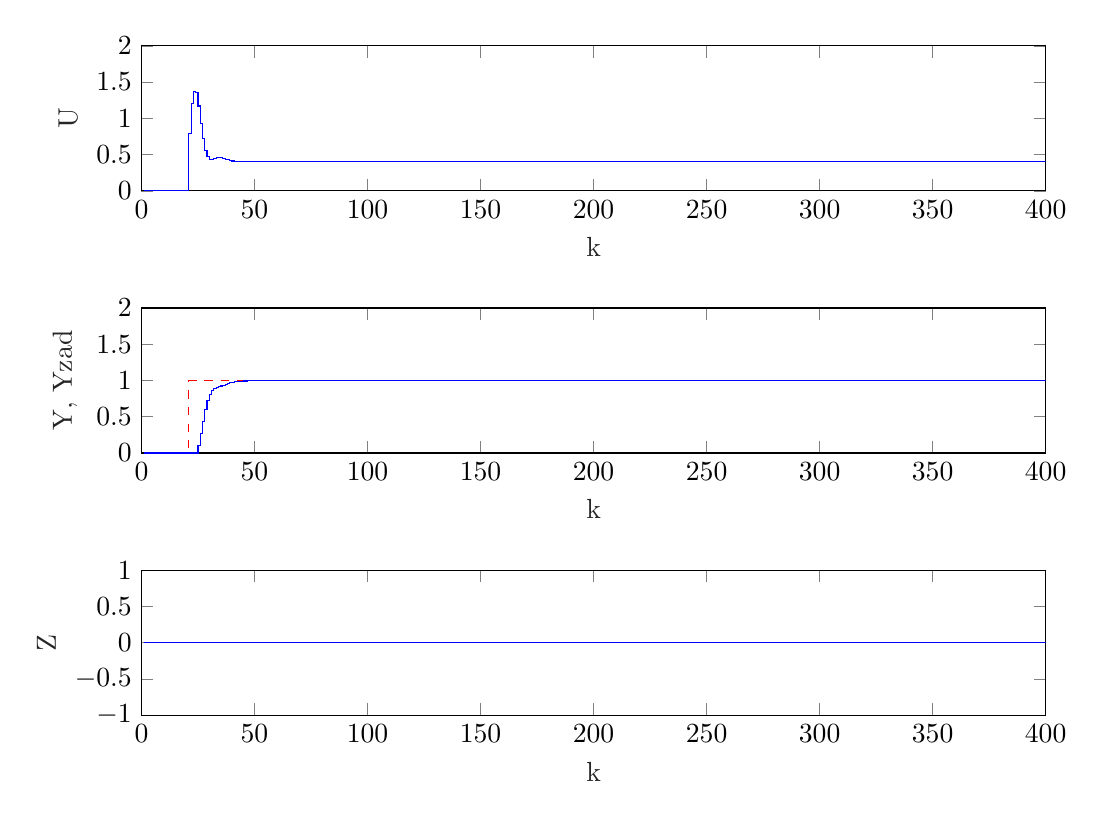
\begin{tikzpicture}

\begin{axis}[%
width=4.521in,
height=0.725in,
at={(0.758in,3.322in)},
scale only axis,
xmin=0,
xmax=400,
xlabel style={font=\color{white!15!black}},
xlabel={k},
ymin=0,
ymax=2,
ylabel style={font=\color{white!15!black}},
ylabel={U},
axis background/.style={fill=white}
]
\addplot[const plot, color=blue, forget plot] table[row sep=crcr] {%
1	0\\
2	0\\
3	0\\
4	0\\
5	0\\
6	0\\
7	0\\
8	0\\
9	0\\
10	0\\
11	0\\
12	0\\
13	0\\
14	0\\
15	0\\
16	0\\
17	0\\
18	0\\
19	0\\
20	0\\
21	0.787678403053571\\
22	1.208742917811\\
23	1.36985186422901\\
24	1.36126435336296\\
25	1.17018885273973\\
26	0.931370878139707\\
27	0.717620992651971\\
28	0.559397468763918\\
29	0.470027290696758\\
30	0.435664891546638\\
31	0.434581642720861\\
32	0.44724172579387\\
33	0.459298333969699\\
34	0.463868456929598\\
35	0.460020954567394\\
36	0.450183599516335\\
37	0.437944991410354\\
38	0.426398904206206\\
39	0.417386139113027\\
40	0.411458836928908\\
41	0.408230575205152\\
42	0.406857900928678\\
43	0.406452250461595\\
44	0.406330298326166\\
45	0.406101786299725\\
46	0.405638637690471\\
47	0.404985093512061\\
48	0.404259991719975\\
49	0.403582129231088\\
50	0.403029747113777\\
51	0.402630630260762\\
52	0.402372064310268\\
53	0.402218930828283\\
54	0.402131022018547\\
55	0.402074797033436\\
56	0.402028511984961\\
57	0.401982049136084\\
58	0.401933736369795\\
59	0.401886330291048\\
60	0.401843641128754\\
61	0.401808457609069\\
62	0.401781775923969\\
63	0.401762965154195\\
64	0.401750396421655\\
65	0.401742138940029\\
66	0.401736482504649\\
67	0.401732202887533\\
68	0.401728598773988\\
69	0.401725383586031\\
70	0.401722522136552\\
71	0.401720079660312\\
72	0.401718118498168\\
73	0.401716649196286\\
74	0.40171562462548\\
75	0.401714958665984\\
76	0.401714552257619\\
77	0.401714315216572\\
78	0.401714178673854\\
79	0.401714098077135\\
80	0.40171404955572\\
81	0.401714023231863\\
82	0.401714016453378\\
83	0.401714028707691\\
84	0.401714058773123\\
85	0.40171410381387\\
86	0.4017141597227\\
87	0.401714221982553\\
88	0.401714286504721\\
89	0.401714350158844\\
90	0.40171441093428\\
91	0.401714467813994\\
92	0.401714520496767\\
93	0.401714569093722\\
94	0.401714613882194\\
95	0.401714655150816\\
96	0.401714693131459\\
97	0.401714727992746\\
98	0.40171475986483\\
99	0.401714788870674\\
100	0.401714815148994\\
101	0.401714838863713\\
102	0.401714860201495\\
103	0.401714879362157\\
104	0.401714896547082\\
105	0.401714911949362\\
106	0.401714925747485\\
107	0.401714938102719\\
108	0.401714949159327\\
109	0.401714959046379\\
110	0.401714967880065\\
111	0.401714975765781\\
112	0.40171498279966\\
113	0.401714989069536\\
114	0.401714994655501\\
115	0.401714999630262\\
116	0.401715004059465\\
117	0.40171500800208\\
118	0.40171501151088\\
119	0.401715014632989\\
120	0.401715017410447\\
121	0.40171501988077\\
122	0.401715022077457\\
123	0.401715024030432\\
124	0.401715025766432\\
125	0.401715027309338\\
126	0.401715028680465\\
127	0.401715029898823\\
128	0.401715030981347\\
129	0.401715031943114\\
130	0.401715032797538\\
131	0.401715033556553\\
132	0.40171503423077\\
133	0.401715034829628\\
134	0.401715035361519\\
135	0.40171503583391\\
136	0.40171503625344\\
137	0.401715036626009\\
138	0.401715036956867\\
139	0.401715037250674\\
140	0.401715037511576\\
141	0.401715037743252\\
142	0.401715037948974\\
143	0.401715038131646\\
144	0.401715038293848\\
145	0.401715038437871\\
146	0.401715038565751\\
147	0.401715038679294\\
148	0.401715038780105\\
149	0.401715038869607\\
150	0.401715038949062\\
151	0.401715039019589\\
152	0.40171503908218\\
153	0.401715039137716\\
154	0.401715039186979\\
155	0.401715039230668\\
156	0.401715039269408\\
157	0.401715039303763\\
158	0.401715039334248\\
159	0.401715039361342\\
160	0.401715039385496\\
161	0.401715039407144\\
162	0.401715039426709\\
163	0.401715039444603\\
164	0.401715039461225\\
165	0.401715039476948\\
166	0.40171503949209\\
167	0.401715039506872\\
168	0.401715039521363\\
169	0.401715039535396\\
170	0.401715039548475\\
171	0.401715039559665\\
172	0.401715039567483\\
173	0.401715039569808\\
174	0.401715039563838\\
175	0.401715039546142\\
176	0.401715039512859\\
177	0.401715039460107\\
178	0.401715039384693\\
179	0.40171503928519\\
180	0.401715039163444\\
181	0.401715039026563\\
182	0.401715038889336\\
183	0.401715038776968\\
184	0.401715038727851\\
185	0.401715038795893\\
186	0.401715039051668\\
187	0.401715039581358\\
188	0.401715040482119\\
189	0.401715041852192\\
190	0.40171504377386\\
191	0.401715046287302\\
192	0.401715049353673\\
193	0.401715052806533\\
194	0.401715056292215\\
195	0.401715059202173\\
196	0.401715060603929\\
197	0.401715059182141\\
198	0.401715053207627\\
199	0.401715040559609\\
200	0.401715018834633\\
201	0.401714985583409\\
202	0.401714938722673\\
203	0.401714877170587\\
204	0.401714801747807\\
205	0.401714716367835\\
206	0.401714629504443\\
207	0.40171455586511\\
208	0.401714518112054\\
209	0.401714548352286\\
210	0.401714688963938\\
211	0.401714992141819\\
212	0.401715517343089\\
213	0.401716325618138\\
214	0.401717469662126\\
215	0.401718978378935\\
216	0.401720834893767\\
217	0.401722947389869\\
218	0.401725113006342\\
219	0.40172697645904\\
220	0.401728235325785\\
221	0.401728735734543\\
222	0.401728498234346\\
223	0.401726336772832\\
224	0.401722494206958\\
225	0.401717815750394\\
226	0.401713217137926\\
227	0.401709689398251\\
228	0.401707761640978\\
229	0.401707437000591\\
230	0.401708346754218\\
231	0.401709913289936\\
232	0.401711573878111\\
233	0.401712930831221\\
234	0.401713800920831\\
235	0.401714194069857\\
236	0.401714242619751\\
237	0.401714119984669\\
238	0.401713977338759\\
239	0.401713909224359\\
240	0.401713948038006\\
241	0.401714078490977\\
242	0.401714260325747\\
243	0.401714449686632\\
244	0.401714613443928\\
245	0.401714734973023\\
246	0.401714812974529\\
247	0.401714856331089\\
248	0.401714878003344\\
249	0.401714890092487\\
250	0.401714901034662\\
251	0.40171491490223\\
252	0.401714932189263\\
253	0.401714951275148\\
254	0.40171496988272\\
255	0.401714986119101\\
256	0.401714998970659\\
257	0.401715008331339\\
258	0.401715014745713\\
259	0.401715019057092\\
260	0.401715022101572\\
261	0.401715024518711\\
262	0.401715026687309\\
263	0.401715028755207\\
264	0.401715030717462\\
265	0.401715032501763\\
266	0.401715034034442\\
267	0.401715035276757\\
268	0.401715036233747\\
269	0.401715036944805\\
270	0.401715037466527\\
271	0.401715037856226\\
272	0.40171503816082\\
273	0.401715038412262\\
274	0.401715038628309\\
275	0.401715038816359\\
276	0.401715038978095\\
277	0.401715039113392\\
278	0.401715039222746\\
279	0.401715039308209\\
280	0.401715039373248\\
281	0.401715039422045\\
282	0.401715039458724\\
283	0.401715039486779\\
284	0.401715039508807\\
285	0.401715039526519\\
286	0.401715039540931\\
287	0.40171503955261\\
288	0.401715039561899\\
289	0.401715039569071\\
290	0.401715039574413\\
291	0.401715039578237\\
292	0.401715039580863\\
293	0.401715039582593\\
294	0.401715039583681\\
295	0.401715039584322\\
296	0.401715039584656\\
297	0.401715039584775\\
298	0.401715039584738\\
299	0.401715039584581\\
300	0.401715039584333\\
301	0.401715039584017\\
302	0.401715039583654\\
303	0.401715039583263\\
304	0.401715039582862\\
305	0.401715039582462\\
306	0.401715039582074\\
307	0.401715039581705\\
308	0.401715039581357\\
309	0.401715039581033\\
310	0.401715039580733\\
311	0.401715039580455\\
312	0.4017150395802\\
313	0.401715039579965\\
314	0.401715039579751\\
315	0.401715039579555\\
316	0.401715039579377\\
317	0.401715039579217\\
318	0.401715039579071\\
319	0.40171503957894\\
320	0.401715039578822\\
321	0.401715039578716\\
322	0.401715039578621\\
323	0.401715039578535\\
324	0.401715039578459\\
325	0.401715039578391\\
326	0.40171503957833\\
327	0.401715039578275\\
328	0.401715039578226\\
329	0.401715039578183\\
330	0.401715039578144\\
331	0.401715039578109\\
332	0.401715039578078\\
333	0.40171503957805\\
334	0.401715039578026\\
335	0.401715039578004\\
336	0.401715039577985\\
337	0.401715039577968\\
338	0.401715039577953\\
339	0.40171503957794\\
340	0.401715039577928\\
341	0.401715039577918\\
342	0.401715039577909\\
343	0.401715039577901\\
344	0.401715039577894\\
345	0.401715039577887\\
346	0.401715039577882\\
347	0.401715039577877\\
348	0.401715039577872\\
349	0.401715039577868\\
350	0.401715039577864\\
351	0.401715039577861\\
352	0.401715039577858\\
353	0.401715039577856\\
354	0.401715039577853\\
355	0.401715039577851\\
356	0.40171503957785\\
357	0.401715039577848\\
358	0.401715039577847\\
359	0.401715039577846\\
360	0.401715039577845\\
361	0.401715039577844\\
362	0.401715039577844\\
363	0.401715039577844\\
364	0.401715039577844\\
365	0.401715039577844\\
366	0.401715039577843\\
367	0.401715039577843\\
368	0.401715039577841\\
369	0.40171503957784\\
370	0.401715039577838\\
371	0.401715039577835\\
372	0.401715039577832\\
373	0.401715039577828\\
374	0.401715039577823\\
375	0.401715039577818\\
376	0.401715039577813\\
377	0.401715039577809\\
378	0.401715039577807\\
379	0.401715039577808\\
380	0.401715039577815\\
381	0.401715039577828\\
382	0.401715039577851\\
383	0.401715039577887\\
384	0.401715039577936\\
385	0.401715039578\\
386	0.401715039578077\\
387	0.401715039578163\\
388	0.40171503957825\\
389	0.401715039578324\\
390	0.401715039578368\\
391	0.401715039578356\\
392	0.401715039578255\\
393	0.401715039578028\\
394	0.401715039577635\\
395	0.401715039577038\\
396	0.401715039576207\\
397	0.40171503957513\\
398	0.401715039573827\\
399	0.401715039572361\\
400	0.401715039570853\\
};
\end{axis}

\begin{axis}[%
width=4.521in,
height=0.725in,
at={(0.758in,2.011in)},
scale only axis,
xmin=0,
xmax=400,
xlabel style={font=\color{white!15!black}},
xlabel={k},
ymin=0,
ymax=2,
ylabel style={font=\color{white!15!black}},
ylabel={Y, Yzad},
axis background/.style={fill=white}
]
\addplot[const plot, color=red, dashed, forget plot] table[row sep=crcr] {%
1	0\\
2	0\\
3	0\\
4	0\\
5	0\\
6	0\\
7	0\\
8	0\\
9	0\\
10	0\\
11	0\\
12	0\\
13	0\\
14	0\\
15	0\\
16	0\\
17	0\\
18	0\\
19	0\\
20	0\\
21	1\\
22	1\\
23	1\\
24	1\\
25	1\\
26	1\\
27	1\\
28	1\\
29	1\\
30	1\\
31	1\\
32	1\\
33	1\\
34	1\\
35	1\\
36	1\\
37	1\\
38	1\\
39	1\\
40	1\\
41	1\\
42	1\\
43	1\\
44	1\\
45	1\\
46	1\\
47	1\\
48	1\\
49	1\\
50	1\\
51	1\\
52	1\\
53	1\\
54	1\\
55	1\\
56	1\\
57	1\\
58	1\\
59	1\\
60	1\\
61	1\\
62	1\\
63	1\\
64	1\\
65	1\\
66	1\\
67	1\\
68	1\\
69	1\\
70	1\\
71	1\\
72	1\\
73	1\\
74	1\\
75	1\\
76	1\\
77	1\\
78	1\\
79	1\\
80	1\\
81	1\\
82	1\\
83	1\\
84	1\\
85	1\\
86	1\\
87	1\\
88	1\\
89	1\\
90	1\\
91	1\\
92	1\\
93	1\\
94	1\\
95	1\\
96	1\\
97	1\\
98	1\\
99	1\\
100	1\\
101	1\\
102	1\\
103	1\\
104	1\\
105	1\\
106	1\\
107	1\\
108	1\\
109	1\\
110	1\\
111	1\\
112	1\\
113	1\\
114	1\\
115	1\\
116	1\\
117	1\\
118	1\\
119	1\\
120	1\\
121	1\\
122	1\\
123	1\\
124	1\\
125	1\\
126	1\\
127	1\\
128	1\\
129	1\\
130	1\\
131	1\\
132	1\\
133	1\\
134	1\\
135	1\\
136	1\\
137	1\\
138	1\\
139	1\\
140	1\\
141	1\\
142	1\\
143	1\\
144	1\\
145	1\\
146	1\\
147	1\\
148	1\\
149	1\\
150	1\\
151	1\\
152	1\\
153	1\\
154	1\\
155	1\\
156	1\\
157	1\\
158	1\\
159	1\\
160	1\\
161	1\\
162	1\\
163	1\\
164	1\\
165	1\\
166	1\\
167	1\\
168	1\\
169	1\\
170	1\\
171	1\\
172	1\\
173	1\\
174	1\\
175	1\\
176	1\\
177	1\\
178	1\\
179	1\\
180	1\\
181	1\\
182	1\\
183	1\\
184	1\\
185	1\\
186	1\\
187	1\\
188	1\\
189	1\\
190	1\\
191	1\\
192	1\\
193	1\\
194	1\\
195	1\\
196	1\\
197	1\\
198	1\\
199	1\\
200	1\\
201	1\\
202	1\\
203	1\\
204	1\\
205	1\\
206	1\\
207	1\\
208	1\\
209	1\\
210	1\\
211	1\\
212	1\\
213	1\\
214	1\\
215	1\\
216	1\\
217	1\\
218	1\\
219	1\\
220	1\\
221	1\\
222	1\\
223	1\\
224	1\\
225	1\\
226	1\\
227	1\\
228	1\\
229	1\\
230	1\\
231	1\\
232	1\\
233	1\\
234	1\\
235	1\\
236	1\\
237	1\\
238	1\\
239	1\\
240	1\\
241	1\\
242	1\\
243	1\\
244	1\\
245	1\\
246	1\\
247	1\\
248	1\\
249	1\\
250	1\\
251	1\\
252	1\\
253	1\\
254	1\\
255	1\\
256	1\\
257	1\\
258	1\\
259	1\\
260	1\\
261	1\\
262	1\\
263	1\\
264	1\\
265	1\\
266	1\\
267	1\\
268	1\\
269	1\\
270	1\\
271	1\\
272	1\\
273	1\\
274	1\\
275	1\\
276	1\\
277	1\\
278	1\\
279	1\\
280	1\\
281	1\\
282	1\\
283	1\\
284	1\\
285	1\\
286	1\\
287	1\\
288	1\\
289	1\\
290	1\\
291	1\\
292	1\\
293	1\\
294	1\\
295	1\\
296	1\\
297	1\\
298	1\\
299	1\\
300	1\\
301	1\\
302	1\\
303	1\\
304	1\\
305	1\\
306	1\\
307	1\\
308	1\\
309	1\\
310	1\\
311	1\\
312	1\\
313	1\\
314	1\\
315	1\\
316	1\\
317	1\\
318	1\\
319	1\\
320	1\\
321	1\\
322	1\\
323	1\\
324	1\\
325	1\\
326	1\\
327	1\\
328	1\\
329	1\\
330	1\\
331	1\\
332	1\\
333	1\\
334	1\\
335	1\\
336	1\\
337	1\\
338	1\\
339	1\\
340	1\\
341	1\\
342	1\\
343	1\\
344	1\\
345	1\\
346	1\\
347	1\\
348	1\\
349	1\\
350	1\\
351	1\\
352	1\\
353	1\\
354	1\\
355	1\\
356	1\\
357	1\\
358	1\\
359	1\\
360	1\\
361	1\\
362	1\\
363	1\\
364	1\\
365	1\\
366	1\\
367	1\\
368	1\\
369	1\\
370	1\\
371	1\\
372	1\\
373	1\\
374	1\\
375	1\\
376	1\\
377	1\\
378	1\\
379	1\\
380	1\\
381	1\\
382	1\\
383	1\\
384	1\\
385	1\\
386	1\\
387	1\\
388	1\\
389	1\\
390	1\\
391	1\\
392	1\\
393	1\\
394	1\\
395	1\\
396	1\\
397	1\\
398	1\\
399	1\\
400	1\\
};
\addplot[const plot, color=blue, forget plot] table[row sep=crcr] {%
1	0\\
2	0\\
3	0\\
4	0\\
5	0\\
6	0\\
7	0\\
8	0\\
9	0\\
10	0\\
11	0\\
12	0\\
13	0\\
14	0\\
15	0\\
16	0\\
17	0\\
18	0\\
19	0\\
20	0\\
21	0\\
22	0\\
23	0\\
24	0\\
25	0.106415352252537\\
26	0.263960851959499\\
27	0.434748826865063\\
28	0.595134021499107\\
29	0.721022005372685\\
30	0.807826205976229\\
31	0.861045816989888\\
32	0.889998481268909\\
33	0.905299103022448\\
34	0.915118394229227\\
35	0.924249798610397\\
36	0.934588214348934\\
37	0.945987702604205\\
38	0.957380200092102\\
39	0.967629508376821\\
40	0.975988802279074\\
41	0.982236429312918\\
42	0.986580673853654\\
43	0.989467233496428\\
44	0.991392277310718\\
45	0.992772908695662\\
46	0.993889689337826\\
47	0.994887924745218\\
48	0.995812705779794\\
49	0.996653923614474\\
50	0.997384679248242\\
51	0.997985475754187\\
52	0.998453899870103\\
53	0.998803695760426\\
54	0.999058414599074\\
55	0.999244069467076\\
56	0.999383532280463\\
57	0.999493678206456\\
58	0.99958502366453\\
59	0.999662972170962\\
60	0.999729685859636\\
61	0.99978583267217\\
62	0.999831809293073\\
63	0.999868355163073\\
64	0.999896677197684\\
65	0.999918287300998\\
66	0.999934744401694\\
67	0.999947432704892\\
68	0.999957436865834\\
69	0.999965517893622\\
70	0.999972160897888\\
71	0.99997765606507\\
72	0.999982180206117\\
73	0.999985859242592\\
74	0.999988805211186\\
75	0.999991130839465\\
76	0.99999294934667\\
77	0.999994367623063\\
78	0.99999547896087\\
79	0.999996358682569\\
80	0.999997063507285\\
81	0.999997633883253\\
82	0.999998097860701\\
83	0.999998475148429\\
84	0.999998780448843\\
85	0.999999025699056\\
86	0.999999221267647\\
87	0.999999376391664\\
88	0.999999499198086\\
89	0.999999596595581\\
90	0.999999674212857\\
91	0.999999736451815\\
92	0.999999786646679\\
93	0.999999827282229\\
94	0.999999860218578\\
95	0.999999886883677\\
96	0.999999908415142\\
97	0.999999925750982\\
98	0.999999939680007\\
99	0.999999950866657\\
100	0.999999959863586\\
101	0.999999967121182\\
102	0.999999972998558\\
103	0.999999977776999\\
104	0.999999981674705\\
105	0.999999984861078\\
106	0.999999987469066\\
107	0.999999989604802\\
108	0.999999991354492\\
109	0.999999992789017\\
110	0.999999993966911\\
111	0.99999999493636\\
112	0.999999995736716\\
113	0.999999996399807\\
114	0.999999996951163\\
115	0.999999997411176\\
116	0.999999997796143\\
117	0.999999998119159\\
118	0.999999998390837\\
119	0.999999998619857\\
120	0.999999998813371\\
121	0.999999998977297\\
122	0.999999999116539\\
123	0.999999999235156\\
124	0.999999999336498\\
125	0.999999999423328\\
126	0.999999999497924\\
127	0.999999999562167\\
128	0.999999999617619\\
129	0.999999999665582\\
130	0.999999999707146\\
131	0.999999999743231\\
132	0.999999999774614\\
133	0.999999999801953\\
134	0.999999999825809\\
135	0.999999999846658\\
136	0.999999999864904\\
137	0.999999999880894\\
138	0.999999999894924\\
139	0.999999999907246\\
140	0.99999999991808\\
141	0.999999999927614\\
142	0.99999999993601\\
143	0.99999999994341\\
144	0.999999999949937\\
145	0.999999999955699\\
146	0.999999999960787\\
147	0.999999999965285\\
148	0.999999999969263\\
149	0.999999999972784\\
150	0.9999999999759\\
151	0.999999999978661\\
152	0.999999999981107\\
153	0.999999999983275\\
154	0.999999999985195\\
155	0.999999999986893\\
156	0.999999999988392\\
157	0.999999999989711\\
158	0.999999999990864\\
159	0.999999999991865\\
160	0.999999999992726\\
161	0.999999999993459\\
162	0.999999999994079\\
163	0.999999999994603\\
164	0.999999999995057\\
165	0.999999999995477\\
166	0.999999999995912\\
167	0.99999999999643\\
168	0.999999999997112\\
169	0.999999999998059\\
170	0.999999999999382\\
171	1.00000000000119\\
172	1.00000000000359\\
173	1.00000000000662\\
174	1.00000000001025\\
175	1.0000000000143\\
176	1.0000000000184\\
177	1.00000000002188\\
178	1.00000000002375\\
179	1.00000000002257\\
180	1.00000000001646\\
181	1.00000000000312\\
182	0.999999999979926\\
183	0.999999999944198\\
184	0.99999999989365\\
185	0.999999999827073\\
186	0.999999999745319\\
187	0.999999999652595\\
188	0.999999999558065\\
189	0.999999999477678\\
190	0.999999999436052\\
191	0.999999999468113\\
192	0.999999999620023\\
193	0.999999999948716\\
194	1.00000000051916\\
195	1.00000000139822\\
196	1.00000000264392\\
197	1.00000000428863\\
198	1.00000000631518\\
199	1.00000000862513\\
200	1.00000001099935\\
201	1.00000001305289\\
202	1.00000001418798\\
203	1.0000000135527\\
204	1.00000001001649\\
205	1.00000000217912\\
206	0.999999988434654\\
207	0.999999967117974\\
208	0.99999993676498\\
209	0.999999896519602\\
210	0.999999846717025\\
211	0.999999789661425\\
212	0.999999730594143\\
213	0.999999678810745\\
214	0.999999648829263\\
215	0.99999966143377\\
216	0.999999744316338\\
217	0.999999931918284\\
218	1.00000026393585\\
219	1.00000078182124\\
220	1.00000152250229\\
221	1.00000250850201\\
222	1.00000373371515\\
223	1.0000051443642\\
224	1.00000664872001\\
225	1.00000813922503\\
226	1.00000951691582\\
227	1.00001052794853\\
228	1.00001096502331\\
229	1.00001074625005\\
230	1.00000991789602\\
231	1.00000865762678\\
232	1.0000072049916\\
233	1.00000578701226\\
234	1.00000456861713\\
235	1.00000362777398\\
236	1.00000296220111\\
237	1.00000251600421\\
238	1.00000221155057\\
239	1.00000197674149\\
240	1.00000176125401\\
241	1.00000154091385\\
242	1.00000131327774\\
243	1.00000108880754\\
244	1.00000088177644\\
245	1.00000070362023\\
246	1.00000055971718\\
247	1.00000044922935\\
248	1.00000036688783\\
249	1.00000030546229\\
250	1.00000025793766\\
251	1.00000021887828\\
252	1.00000018489354\\
253	1.00000015441126\\
254	1.00000012708428\\
255	1.0000001031346\\
256	1.0000000828392\\
257	1.00000006624134\\
258	1.00000005307442\\
259	1.00000004283071\\
260	1.00000003489311\\
261	1.00000002866372\\
262	1.00000002365067\\
263	1.00000001950273\\
264	1.00000001600078\\
265	1.00000001302405\\
266	1.00000001050958\\
267	1.00000000841791\\
268	1.00000000671111\\
269	1.00000000534362\\
270	1.00000000426246\\
271	1.00000000341236\\
272	1.00000000274176\\
273	1.00000000220726\\
274	1.00000000177552\\
275	1.00000000142278\\
276	1.00000000113294\\
277	1.00000000089512\\
278	1.00000000070147\\
279	1.00000000054558\\
280	1.00000000042165\\
281	1.00000000032419\\
282	1.00000000024811\\
283	1.00000000018887\\
284	1.00000000014267\\
285	1.00000000010649\\
286	1.00000000007805\\
287	1.00000000005568\\
288	1.00000000003815\\
289	1.00000000002454\\
290	1.00000000001413\\
291	1.00000000000632\\
292	1.0000000000006\\
293	0.999999999996518\\
294	0.999999999993699\\
295	0.999999999991835\\
296	0.99999999999068\\
297	0.999999999990047\\
298	0.999999999989796\\
299	0.999999999989822\\
300	0.999999999990049\\
301	0.99999999999042\\
302	0.99999999999089\\
303	0.999999999991424\\
304	0.999999999991994\\
305	0.999999999992577\\
306	0.999999999993156\\
307	0.99999999999372\\
308	0.99999999999426\\
309	0.99999999999477\\
310	0.999999999995248\\
311	0.999999999995693\\
312	0.999999999996105\\
313	0.999999999996484\\
314	0.999999999996832\\
315	0.99999999999715\\
316	0.999999999997439\\
317	0.999999999997703\\
318	0.999999999997941\\
319	0.999999999998156\\
320	0.999999999998351\\
321	0.999999999998526\\
322	0.999999999998683\\
323	0.999999999998824\\
324	0.999999999998951\\
325	0.999999999999064\\
326	0.999999999999166\\
327	0.999999999999257\\
328	0.999999999999338\\
329	0.99999999999941\\
330	0.999999999999475\\
331	0.999999999999533\\
332	0.999999999999585\\
333	0.999999999999631\\
334	0.999999999999672\\
335	0.999999999999708\\
336	0.99999999999974\\
337	0.999999999999769\\
338	0.999999999999794\\
339	0.999999999999817\\
340	0.999999999999837\\
341	0.999999999999854\\
342	0.99999999999987\\
343	0.999999999999884\\
344	0.999999999999896\\
345	0.999999999999907\\
346	0.999999999999917\\
347	0.999999999999926\\
348	0.999999999999934\\
349	0.999999999999941\\
350	0.999999999999947\\
351	0.999999999999952\\
352	0.999999999999957\\
353	0.999999999999962\\
354	0.999999999999966\\
355	0.99999999999997\\
356	0.999999999999973\\
357	0.999999999999976\\
358	0.999999999999978\\
359	0.99999999999998\\
360	0.999999999999982\\
361	0.999999999999984\\
362	0.999999999999985\\
363	0.999999999999986\\
364	0.999999999999987\\
365	0.999999999999988\\
366	0.999999999999989\\
367	0.999999999999991\\
368	0.999999999999992\\
369	0.999999999999993\\
370	0.999999999999995\\
371	0.999999999999996\\
372	0.999999999999997\\
373	0.999999999999997\\
374	0.999999999999998\\
375	0.999999999999998\\
376	0.999999999999998\\
377	0.999999999999997\\
378	0.999999999999996\\
379	0.999999999999994\\
380	0.999999999999991\\
381	0.999999999999988\\
382	0.999999999999985\\
383	0.999999999999983\\
384	0.999999999999981\\
385	0.999999999999982\\
386	0.999999999999985\\
387	0.999999999999993\\
388	1.00000000000001\\
389	1.00000000000003\\
390	1.00000000000006\\
391	1.0000000000001\\
392	1.00000000000015\\
393	1.00000000000021\\
394	1.00000000000027\\
395	1.00000000000033\\
396	1.00000000000037\\
397	1.00000000000038\\
398	1.00000000000033\\
399	1.0000000000002\\
400	0.999999999999971\\
};
\end{axis}

\begin{axis}[%
width=4.521in,
height=0.725in,
at={(0.758in,0.7in)},
scale only axis,
xmin=0,
xmax=400,
xlabel style={font=\color{white!15!black}},
xlabel={k},
ymin=-1,
ymax=1,
ylabel style={font=\color{white!15!black}},
ylabel={Z},
axis background/.style={fill=white}
]
\addplot[const plot, color=blue, forget plot] table[row sep=crcr] {%
1	0\\
2	0\\
3	0\\
4	0\\
5	0\\
6	0\\
7	0\\
8	0\\
9	0\\
10	0\\
11	0\\
12	0\\
13	0\\
14	0\\
15	0\\
16	0\\
17	0\\
18	0\\
19	0\\
20	0\\
21	0\\
22	0\\
23	0\\
24	0\\
25	0\\
26	0\\
27	0\\
28	0\\
29	0\\
30	0\\
31	0\\
32	0\\
33	0\\
34	0\\
35	0\\
36	0\\
37	0\\
38	0\\
39	0\\
40	0\\
41	0\\
42	0\\
43	0\\
44	0\\
45	0\\
46	0\\
47	0\\
48	0\\
49	0\\
50	0\\
51	0\\
52	0\\
53	0\\
54	0\\
55	0\\
56	0\\
57	0\\
58	0\\
59	0\\
60	0\\
61	0\\
62	0\\
63	0\\
64	0\\
65	0\\
66	0\\
67	0\\
68	0\\
69	0\\
70	0\\
71	0\\
72	0\\
73	0\\
74	0\\
75	0\\
76	0\\
77	0\\
78	0\\
79	0\\
80	0\\
81	0\\
82	0\\
83	0\\
84	0\\
85	0\\
86	0\\
87	0\\
88	0\\
89	0\\
90	0\\
91	0\\
92	0\\
93	0\\
94	0\\
95	0\\
96	0\\
97	0\\
98	0\\
99	0\\
100	0\\
101	0\\
102	0\\
103	0\\
104	0\\
105	0\\
106	0\\
107	0\\
108	0\\
109	0\\
110	0\\
111	0\\
112	0\\
113	0\\
114	0\\
115	0\\
116	0\\
117	0\\
118	0\\
119	0\\
120	0\\
121	0\\
122	0\\
123	0\\
124	0\\
125	0\\
126	0\\
127	0\\
128	0\\
129	0\\
130	0\\
131	0\\
132	0\\
133	0\\
134	0\\
135	0\\
136	0\\
137	0\\
138	0\\
139	0\\
140	0\\
141	0\\
142	0\\
143	0\\
144	0\\
145	0\\
146	0\\
147	0\\
148	0\\
149	0\\
150	0\\
151	0\\
152	0\\
153	0\\
154	0\\
155	0\\
156	0\\
157	0\\
158	0\\
159	0\\
160	0\\
161	0\\
162	0\\
163	0\\
164	0\\
165	0\\
166	0\\
167	0\\
168	0\\
169	0\\
170	0\\
171	0\\
172	0\\
173	0\\
174	0\\
175	0\\
176	0\\
177	0\\
178	0\\
179	0\\
180	0\\
181	0\\
182	0\\
183	0\\
184	0\\
185	0\\
186	0\\
187	0\\
188	0\\
189	0\\
190	0\\
191	0\\
192	0\\
193	0\\
194	0\\
195	0\\
196	0\\
197	0\\
198	0\\
199	0\\
200	0\\
201	0\\
202	0\\
203	0\\
204	0\\
205	0\\
206	0\\
207	0\\
208	0\\
209	0\\
210	0\\
211	0\\
212	0\\
213	0\\
214	0\\
215	0\\
216	0\\
217	0\\
218	0\\
219	0\\
220	0\\
221	0\\
222	0\\
223	0\\
224	0\\
225	0\\
226	0\\
227	0\\
228	0\\
229	0\\
230	0\\
231	0\\
232	0\\
233	0\\
234	0\\
235	0\\
236	0\\
237	0\\
238	0\\
239	0\\
240	0\\
241	0\\
242	0\\
243	0\\
244	0\\
245	0\\
246	0\\
247	0\\
248	0\\
249	0\\
250	0\\
251	0\\
252	0\\
253	0\\
254	0\\
255	0\\
256	0\\
257	0\\
258	0\\
259	0\\
260	0\\
261	0\\
262	0\\
263	0\\
264	0\\
265	0\\
266	0\\
267	0\\
268	0\\
269	0\\
270	0\\
271	0\\
272	0\\
273	0\\
274	0\\
275	0\\
276	0\\
277	0\\
278	0\\
279	0\\
280	0\\
281	0\\
282	0\\
283	0\\
284	0\\
285	0\\
286	0\\
287	0\\
288	0\\
289	0\\
290	0\\
291	0\\
292	0\\
293	0\\
294	0\\
295	0\\
296	0\\
297	0\\
298	0\\
299	0\\
300	0\\
301	0\\
302	0\\
303	0\\
304	0\\
305	0\\
306	0\\
307	0\\
308	0\\
309	0\\
310	0\\
311	0\\
312	0\\
313	0\\
314	0\\
315	0\\
316	0\\
317	0\\
318	0\\
319	0\\
320	0\\
321	0\\
322	0\\
323	0\\
324	0\\
325	0\\
326	0\\
327	0\\
328	0\\
329	0\\
330	0\\
331	0\\
332	0\\
333	0\\
334	0\\
335	0\\
336	0\\
337	0\\
338	0\\
339	0\\
340	0\\
341	0\\
342	0\\
343	0\\
344	0\\
345	0\\
346	0\\
347	0\\
348	0\\
349	0\\
350	0\\
351	0\\
352	0\\
353	0\\
354	0\\
355	0\\
356	0\\
357	0\\
358	0\\
359	0\\
360	0\\
361	0\\
362	0\\
363	0\\
364	0\\
365	0\\
366	0\\
367	0\\
368	0\\
369	0\\
370	0\\
371	0\\
372	0\\
373	0\\
374	0\\
375	0\\
376	0\\
377	0\\
378	0\\
379	0\\
380	0\\
381	0\\
382	0\\
383	0\\
384	0\\
385	0\\
386	0\\
387	0\\
388	0\\
389	0\\
390	0\\
391	0\\
392	0\\
393	0\\
394	0\\
395	0\\
396	0\\
397	0\\
398	0\\
399	0\\
400	0\\
};
\end{axis}
\end{tikzpicture}%
	\label{run}
\end{figure}

Dla dobranych parametrów $D$~=~$N$~=~201, $N_u$~=~4, $\lambda$~=~\num{1} wykonano wizualizację przebiegu (Rys. \ref{run} )

